

\fancypagestyle{miEstilo5}{
   \lhead{5. Descripción de la aplicación}
   %\chead{1. Introducción}
   \rhead{Página \thepage}
   \lfoot{}
   \cfoot{}
   \rfoot{}
}

\pagestyle{miEstilo5}

\section{Descripción de la aplicación: SIVIRA}

El sistema de videovigilancia con una Raspberry PI (\texttt{SIVIRA}) es una aplicación que nos permite construir un sistema de seguridad basado en la videovigilancia de bajo coste utilizando una Raspberry PI , una cámara y un sensor de movimiento.

La idea es poder controlar el sistema a través de una aplicación móvil, con la que el usuario pueda conectarse desde cualquier parte y tener acceso a su información y sistema de seguridad. Las funciones principales de este sistema son las siguientes:

\begin{itemize}
\item \textbf{Sistema automático} de alertas generadas al capturar el movimiento.
\item \textbf{Sistema manual} para grabar vídeo o capturar una foto instantáneamente.   
\item \textbf{Sistema de streaming} para visualizar la imagen en tiempo real.
\end{itemize}

Además, podemos realizar configuraciones personalizadas a la cámara, como por ejemplo, cambiar la resolución, rotación... y la opción de poder activar un agente que filtre las alertas automáticas, generando únicamente alertas cuando se detecta a una persona en una imagen (evitar falsos positivos).

\subsection{Arquitectura de la aplicación}

Esta aplicación consta de una \textbf{arquitectura basada en microservicios}. Una arquitectura de microservicios \cite{ref25} consta de una colección de servicios autónomos y pequeños. Los servicios son independientes entre sí y cada uno debe implementar una funcionalidad de negocio individual.

En cierto modo, los microservicios son la evolución natural de las arquitecturas orientadas a servicios aunque con ciertas diferencias.

\newpage

\textbf{¿Por qué se ha utilizado esta arquitectura?}

En primer lugar, se ha realizado una descomposición de los principales componentes necesarios para construir la aplicación, y se ha observado que hay funcionalidades independientes que se pueden comunicar entre sí para integrarse en la aplicación. Esto aporta una gran serie de ventajas respecto a un diseño monolítico \cite{ref26} como las siguientes:

\begin{itemize}
\item \textbf{Implementaciones independientes}: Es posible actualizar un servicio sin volver a implementar toda la aplicación y revertir o poner al día una actualización si algo va mal. Las correcciones de errores y las publicaciones de características son más fáciles de administrar y entrañan menos riesgo, por lo tanto, facilitan el mantenimiento de este software.

\item \textbf{Desarrollo independiente}: Cada microservicio se ha ido desarrollando a lo largo de una iteración y de forma independiente al resto. Esto ha agilizado bastante la tarea, ya que las modificaciones y errores no se retropropagaban.

\item \textbf{Fácil escalabilidad}: Cada microservicio puede ser escalado de forma independiente al resto. Por ejemplo, en el caso de que sea necesario escalar la detección de objetos en imágenes, bastaría con replicar el microservicio de detección de objetos y balancear las peticiones entre ellos.

\item \textbf{Fácil integración y alta cohesión}: Un sistema de microservicios se puede integrar y adaptar a casi cualquier sistema. Por ejemplo, en el caso de que quisiera añadir un sistema multicámara a la aplicación, bastaría con añadir una nueva capa superior de abstracción sobre el software desarrollado y se integraría perfectamente.
\end{itemize}

Basándome en esta arquitectura basada en microservicios, se ha diseñado el siguiente sistema (ver figura \ref{img:arquitectura}).

\newpage

\begin{figure}[h]
	\centering
	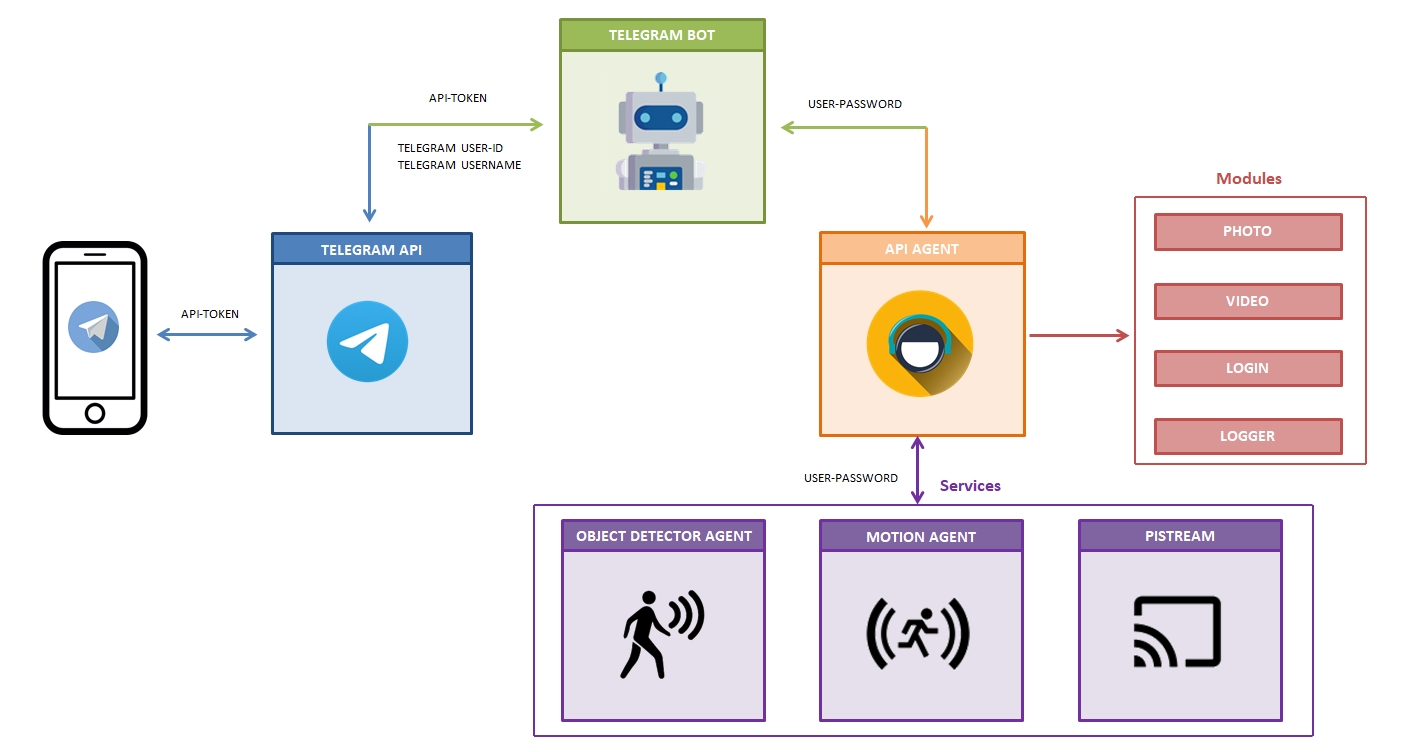
\includegraphics[scale=0.4]{images/23}
	\caption{Arquitectura de la aplicación}
	\label{img:arquitectura}
\end{figure}

En primer lugar tenemos los \textbf{módulos} de la aplicación (ver figura \ref{img:modulos}) que implementan un conjunto de funcionalidades para comunicarse con el módulo hardware de la cámara de la Raspberry PI, autenticación y logs.

\begin{figure}[h]
	\centering
	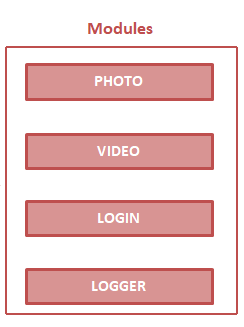
\includegraphics[scale=0.4]{images/24}
	\caption{Módulos de la aplicación}
	\label{img:modulos}
\end{figure}

A continuación tenemos el \textbf{API agent} (ver figura \ref{img:api}). Este es un servicio web que inicia la API que conecta con el resto de módulos de la aplicación.

\begin{figure}[h]
	\centering
	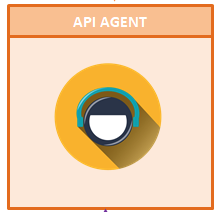
\includegraphics[scale=0.35]{images/25}
	\caption{API agent}
	\label{img:api}
\end{figure}

\newpage

Esta API importa y hace uso de los módulos de la aplicación. 

\begin{figure}[h]
	\centering
	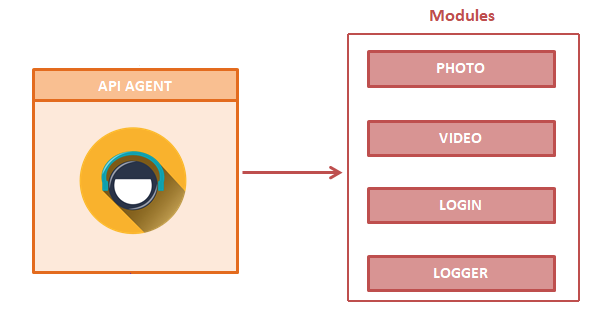
\includegraphics[scale=0.35]{images/27}
	\caption{Conexión entre la API y los módulos}
	\label{img:conexionapimodulos}
\end{figure}

Por otra parte, tenemos un conjunto de servicios que se inician de forma independiente y proporcionan las funcionalidades de detección de objetos en imágenes, detección de movimiento y servicio de streaming.

\begin{figure}[h]
	\centering
	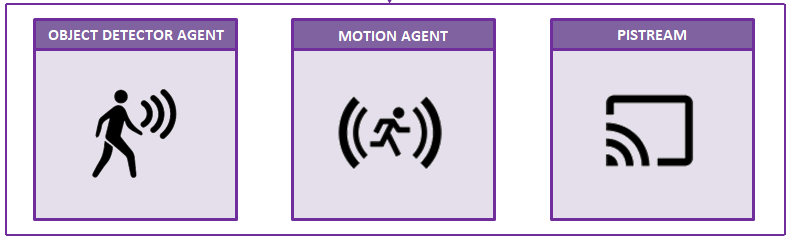
\includegraphics[scale=0.35]{images/26}
	\caption{Servicios de la aplicación}
	\label{img:serviciosaplicacion}
\end{figure}

La API está conectada con todo este conjunto de servicios y tiene la capacidad de poder gestionarlos.

\begin{figure}[h]
	\centering
	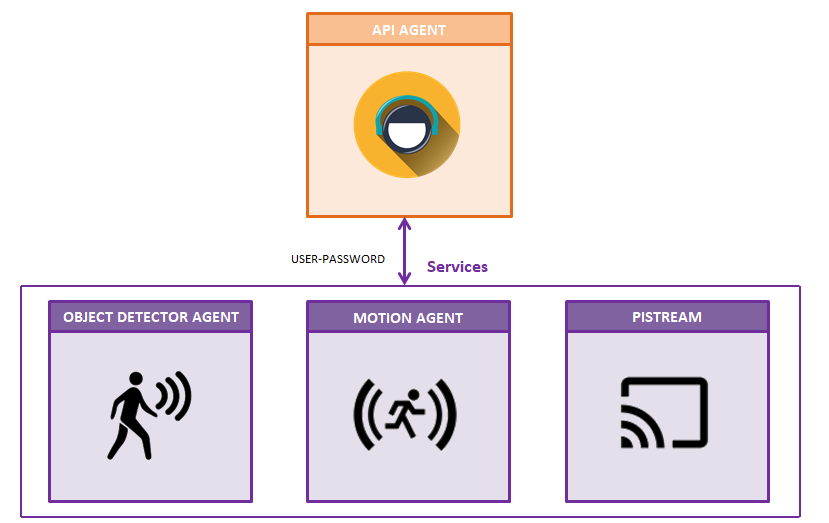
\includegraphics[scale=0.35]{images/28}
	\caption{Conexión entre los servicios y la API}
	\label{img:conexionserviciosapi}
\end{figure}

En la figura \ref{img:conexionmodulosserviciosapi} podemos ver, como quedan unidos todos estos componentes entre sí.

\newpage


\begin{figure}[h]
	\centering
	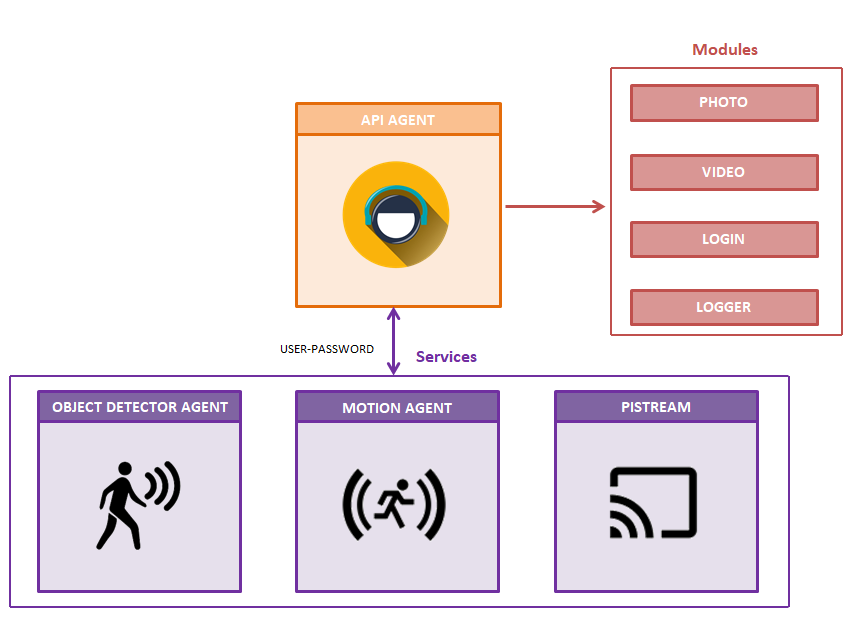
\includegraphics[scale=0.35]{images/35}
	\caption{Conexión de módulos y servicios con la API}
	\label{img:conexionmodulosserviciosapi}
\end{figure}

El siguiente componente es el \textbf{bot de Telegram}. Este bot es un proceso que se ejecuta junto a la API, cuyo objetivo es conectar la API de telegram con la API de la aplicación.

\begin{figure}[h]
	\centering
	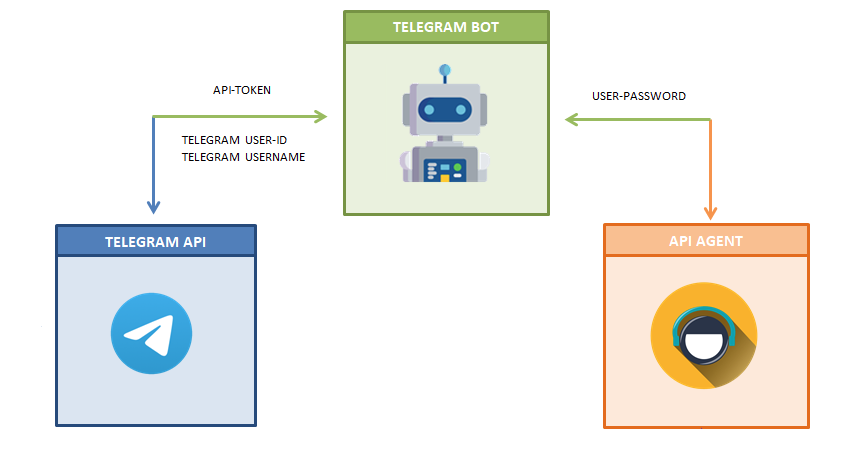
\includegraphics[scale=0.35]{images/34}
	\caption{Conexión entre el bot de telegram y la API}
	\label{img:conexionbotapitelegram}
\end{figure}

Finalmente, el usuario puede interactuar con la aplicación (\texttt{SIVIRA}), haciendo uso de la aplicación multiplataforma \texttt{Telegram}, usando el bot que se ha creado.

\begin{figure}[h]
	\centering
	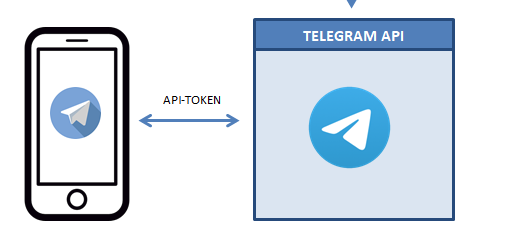
\includegraphics[scale=0.35]{images/33}
	\caption{Conexión entre el usuario y la aplicación}
	\label{img:usuariotelegram}
\end{figure}

\newpage

\subsection{Descripción de los componentes}

La aplicación (SIVIRA) desarrollada en este proyecto está compuesta por los siguientes componentes:

\subsubsection{Módulos}

Los módulos son un conjunto de funciones cuyo objetivo es encapsular funcionalidades que después serán utilizadas por el resto de componentes de la aplicación (ver figura \ref{img:modulos}). A continuación se realiza una descripción de cada uno de ellos.

\textbf{Logger}

Módulo cuyo objetivo es poder capturar y almacenar los logs de la aplicación en ficheros independientes para monitorizar el estado de la aplicación. Su implementación parte de una clase abstracta base, cuyo objetivo es definir las propiedades y métodos que tendrán todas las clases que implementarán los logs del sistema. 


PONER AQUÍ DIAGRAMA DE CLASES DE LOGS

\newpage

Por defecto, los logs son mostrados y almacenados de la siguiente forma:

\begin{itemize}
\item \textbf{Consola}: Corresponde a la salida \texttt{stdout}. Todo logs por encima de un nivel determinado de prioridad será mostrado por la salida de consola.

\item \textbf{Archivo de módulo}: Cada módulo y microservicio tendrán un fichero de log independiente para poder monitorizar su comportamiento a lo largo de su ejecución.

\item \textbf{Archivo de la aplicación}: La aplicación consta de un archivo de logs donde se almacenan todos los logs de módulos y microservicios de forma conjunta.

\item \textbf{Archivo de errores}: Todos los errores que surjan en cualquier módulo o microservicio es almacenado en este fichero para poder comprobar el estado de la aplicación.

\end{itemize}

Los niveles de logs que se han establecido son los siguientes:

\begin{itemize}

\item \textbf{DEBUG}: Nivel destinado a la depuración del código. Este nivel solo genera log en la salida por pantalla, y no se almacena en ningún fichero.

\item \textbf{INFO}: Nivel destinado a mostrar un mensaje informativo sobre alguna acción llevada a cabo. Estos logs son almacenados en el fichero de módulo correspondiente, en el fichero de logs de la aplicación y mostrados por pantalla.

\item \textbf{WARNING}: Nivel destinado a mostrar un mensajes de advertencia por posible mal uso de las llamadas a funciones, o simplemente porque algunas de ellas están '{deprecated}`. Estos logs son almacenados en el fichero de módulo correspondiente, en el fichero de logs de la aplicación y mostrados por pantalla.

\item \textbf{ERROR}: Nivel destinado a mostrar mensajes de error, que no son críticos para el sistema, y por lo tanto la aplicación sigue ejecutándose a pesar de producirse dichos error. Estos logs son almacenados en el fichero de módulo correspondiente, en el fichero de logs de la aplicación, en el fichero de errores de la aplicación.

\item \textbf{CRITICAL}: Nivel destinado a mostrar mensajes de error críticos que provocan el fallo de la aplicación. Estos logs son almacenados en el fichero de módulo correspondiente, en el fichero de logs de la aplicación, en el fichero de errores de la aplicación.

\end{itemize}



El formato por defecto de los logs es el siguiente:

\begin{itemize}
\item \textbf{Formato del archivo de errores}: \texttt{[Nivel:FechaHora:NombreArchivo:Función:Línea] Mensaje}. Por ejemplo:

\vspace{-1cm}

\begin{verbatim}

[ERROR:2019-08-15 13:10:11,597:logger.py:error:112x = set] Error while
trying to send an alert to Detector API agent with address 
http://192.168.1.100:11000.¿It is running?

\end{verbatim}


\vspace{-1cm}

\item \textbf{Formato del resto de logs}: \texttt{[Nivel:FechaHora] Mensaje}. Por ejemplo:

\vspace{-1.2cm}

\begin{verbatim}

[INFO:2019-08-13 18:35:03,278] A 5 seconds video is being 

\end{verbatim}

\end{itemize}

\vspace{-1.2cm}

Todos los ficheros de logs son almacenados en el directorio llamado \texttt{logs}. Dentro de dicho directorio, nos encontraremos los siguientes ficheros de logs:

\vspace{-0.4cm}

\begin{itemize}
\item \textbf{API\_agent.log}: Logs correspondientes a la API.
\item \textbf{detector\_object\_agent.log}: Logs correspondientes al agente detector de objetos.
\item \textbf{photo\_module.log}: Logs correspondientes al módulo de fotos.
\item \textbf{video\_module.log}: Logs correspondientes al módulo de vídeo.
\item \textbf{motion\_agent.log}: Logs correspondientes al agente detector de movimiento.
\item \textbf{security\_system\_PI\_app\_ERROR.log}: Logs correspondientes a los errores obtenidos por cualquier módulo o microservicio.
\item \textbf{security\_system\_PI\_app.log}: Logs correspondientes a los generados por módulos y microservicios a lo largo de su ejecución.
\item \textbf{telegram\_bot\_agent.log}: Logs correspondientes al bot de telegram.

\end{itemize}

La implementación de este módulo puede comprobarse en este \href{https://github.com/jmv74211/TFM_security_system_PI/blob/master/src/modules/logger.py}{enlace}.

\textbf{Photo} 

Módulo que implementa la clase \texttt{Photo} con la que se pretende administrar el recurso de la cámara de la Raspberry PI para capturar fotografías, además de establecer los diferentes parámetros de la cámara como resolución, rotación \ldots

Esta clase añade una capa de abstracción a la biblioteca \texttt{PiCamera} \cite{ref12}, para permitir conectarse con el recurso de la cámara de forma personalizada.

Las funcionalidades que aporta este módulo son las siguientes:

\vspace{-0.5cm}

\begin{itemize}
\item Capturar una fotografía.
\item Realizar una captura secuencial de fotografías en un intervalo de tiempo
\item Establecer la configuración de la cámara: Rotación, resolución, giro horizontal o giro vertical.

\end{itemize}

\vspace{-0.5cm}

La implementación de este módulo puede comprobarse en este \href{https://github.com/jmv74211/TFM_security_system_PI/blob/master/src/modules/photo.py}{enlace}.

\textbf{Video} 

Módulo que implementa la clase \texttt{Video} con la que se pretende administrar el recurso de la cámara de la Raspberry PI para realizar grabaciones de vídeo, además de establecer los diferentes parámetros de la cámara como resolución, rotación \ldots

Esta clase añade una capa de abstracción a la biblioteca \texttt{PiCamera} \cite{ref12}, para permitir conectarse con el recurso de la cámara de vídeo de forma personalizada.

Las funcionalidades que aporta este módulo son las siguientes:

\vspace{-0.5cm}

\begin{itemize}
\item Realizar una grabación de vídeo.
\item Conversión de formato de vídeo \texttt{.h264} a \texttt{.mp4} (compatible con telegram).
\item Establecer la configuración: Rotación, resolución, giro horizontal, giro vertical y mostrar hora y fecha durante la grabación de vídeo. .

\end{itemize}

\vspace{-0.5cm}

La implementación de este módulo puede comprobarse en este \href{https://github.com/jmv74211/TFM_security_system_PI/blob/master/src/modules/video.py}{enlace}.

\textbf{Authentication} 

Módulo implementado para realizar una autenticación en el sistema. Esta autenticación es solicitada por la API, ya que junto a la petición deberá de ir las credenciales de acceso que se han definido en la configuración de la aplicación.

Este módulo básicamente implementa una función para poder comprobar si la autenticación es correcta. Su implementación puede comprobarse en este \href{https://github.com/jmv74211/TFM_security_system_PI/blob/master/src/modules/authentication.py}{enlace}.

\subsubsection{Servicios}

Los servicios son procesos destinados a realizar alguna tarea en concreto y enviar una petición o respuesta con los resultados a la API. A continuación se realiza una descripción de cada uno de ellos.

\textbf{Motion agent}

Este servicio se encarga de controlar el sensor de movimiento y detectar cuando es activado para poder manejar dicho evento y enviar una alerta a la API. Las tareas realizadas por este servicio son las siguientes:

\vspace{-0.5cm}

\begin{itemize}
\item Controlar el estado del sensor.
\item Capturar fotos o vídeos en caso de detectar algún tipo de movimiento.
\item Enviar una petición para procesar la imagen capturada, con objetivo de poder detectar si hay alguna persona en ella.
\item Generar una alerta en la API en caso detectar a una persona en la foto.
\item Mover la foto generada por la alerta al directorio de \texttt{false\_positive} en caso de no detectar ninguna persona en la foto.

\end{itemize}

Para más información, en la sección X se detallará como funciona e interacciona este servicio con el resto de elementos.

La implementación de este servicio puede comprobarse en este \href{https://github.com/jmv74211/TFM_security_system_PI/blob/master/src/agents/motion_agent.py}{enlace}.

\textbf{Object detector agent}

Este servicio se encarga de procesar una foto y devolver una lista de objetos detectadas en dicha foto. Este servicio es usado por el \texttt{motion agent}, ya que cuando detecta movimiento (si la funcionalidad de detección de personas está activada), envía una petición a este servicio, y se le responde con la lista de objetos.

Esta funcionalidad ha sido implementada gracias al uso de la biblioteca de aprendizaje automático \texttt{Tensorflow} \cite{ref17}, ya que se ha utilizado para cargar el modelo preentrenado \texttt{ssdlite\_mobilenet\_v2\_coco} \cite{ref27} para poder predecir una lista de objetos que aparecen en una imagen.

El motivo por el cual se ha seleccionado ese modelo, es porque es el modelo más ligero, y el único viable para este proyecto en la Raspberry PI (debido a sus bajos recursos hardware). Antes de escoger este modelo, se hicieron pruebas con otros un poco más pesados y los resultados eran abrumadores. Utilizando otros modelos, se han obtenido una media de espera de más de 100 segundos para procesar la imagen (obviamente inviable).

Utilizar el modelo \texttt{ssdlite\_mobilenet\_v2\_coco} junto con una resolución de imagen media (1280x720) ha permitido obtener tiempos de procesamiento comprendidos entre unos 5 y 10 segundos, tiempo de espera que es aceptable.

El uso de este servicio es optativo, es decir, puede ser deshabilitado en las opciones o mediante la intefaz de usuario, y la aplicación puede funcionar normalmente. Es optativo por el hecho de su uso implica una serie de ventajas e inconvenientes que puede hacer pensar si realmente vale la pena utilizar este servicio o no.

Personalmente, yo recomendaría usar este servicio, ya que hay casos en los que se quiere controlar una zona y puede que haya demasiadas falsos positivos en las alertas por motivos como: animales domésticos, alta sensibilidad del sensor \ldots

A continuación se mencionan las posibles ventajas e inconvenientes de utilizar este servicio.

Ventajas

\begin{itemize}

\vspace{-0.5cm}

\item Evita posibles falsos positivos en las alertas generadas.
\item Puede aumentar el grado de eficacia del sistema de seguridad.
\end{itemize}

Desventajas

\vspace{-0.5cm}

\begin{itemize}
\item Añade sobrecarga de procesamiento en la Raspberry PI, calentamiento \ldots.
\item Añade latencia (5 a 10 segundos) en el momento de generar alertas, es decir, aumenta el tiempo desde que se produce un evento hasta que se envía la alerta.
\item Dado que el modelo de predicción es muy ligero, no es efectivo al 100\% y puede cometer algunos fallos.
\item Dificulta el proceso de instalación de la aplicación.
\end{itemize}

Por estos motivos, y porque la instalación de este agente puede resultar un poco tediosa (aunque todo está explicado en el repositorio del proyecto \cite{ref1}) se ha decidido entre realizar dos tipos de instalaciones de la aplicación, una en la que se utiliza otro servicio para filtrar eventos y reducir el número de falsos positivos en las alertas, y la otra en la que se prescinde totalmente de este servicio, y se genera una alerta tras la detección de cualquier movimiento.

La implementación de este servicio puede comprobarse en este \href{https://github.com/jmv74211/TFM_security_system_PI/blob/master/src/agents/object_detector_agent.py}{enlace}.



